\subsection{Architecture hybride}
\begin{figure}[h]
	\centering
		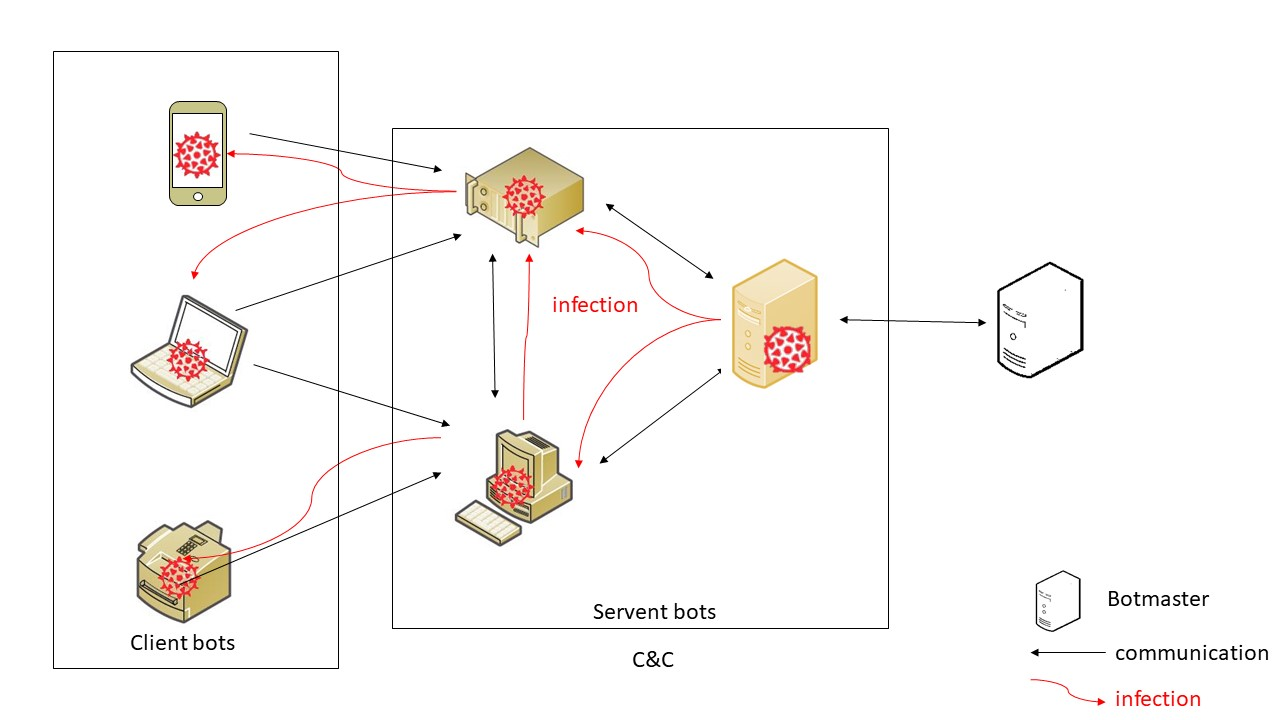
\includegraphics[width=0.75\textwidth]{structure_hybride_P2P}
	\label{fig:hybridep2p}
	\caption[Structure hybride P2P]{Structure hybride P2P}
\end{figure}

\subsubsection{Définition}
Une architecture hybride intègre une solution de repli, comme à l'aide d'un DGA\footnote{Domain Generation Algorithm} ou de plusieurs niveaux successifs entre le P2P et le C\&C.Cette hiérarchie permet de masquer une partie des adresses IP utilisées afin de rendre plus complexe l'analyse du botnet.
L'association de bot clients et de bots servent\footnote{serv-\textbf{eur} et cli-\textbf{ent}} met en évidence l'organisation du réseau par le botmaster.
Ces niveaux intermédiaires permettent de solidifier l'architecture du réseau.

\subsubsection{Liste des protocoles utilisés par le botnet}
Reprenant les protocoles présentés dans les architectures précédentes, L'efficacité, la furtivité et la complexité des méthodes de communication ont pour objectif de nuire aux efforts de démantèlement.
Ainsi, les coopérations internationales entre acteurs institutionnels et
privés sont généralement nécessaires pour permettre de démanteler les botnets les plus sophistiqués.

\subsubsection{Avantages}
\begin{itemize}
	\item Nombre important de domaines
  \item masquage de l'adresse IP
\end{itemize}

\subsubsection{Inconvénients}
\begin{itemize}
	\item tributaire de la bande passante
\end{itemize}

%--------------------------------------------------------------------
%ajouter un botnet
%glisser le .csv dans le dossier exemples de la section 2
%inclure la ligne \csvautotabular[respect all]{Section/2-Ssection/exemples/nom-du-botnet}
%--------------------------------------------------------------------

\subsubsection{exemples}
\noindent
\resizebox{\textwidth}{!}{
\csvautotabular[respect all]{Section/2-Ssection/exemples/Gameover-Zeus.csv}
}
\resizebox{\textwidth}{!}{
\csvautotabular[respect all]{Section/2-Ssection/exemples/Mirai.csv}
}